
%%%%%%%%%%%%%%%%%%%%%%%%%%%%%%%%%%%%%%%%%% FIGURE
\begin{figure*}[tb]   
  \begin{center}
   \vspace{-0mm}
   %\includegraphics[width=0.23\textwidth]{figs/model}
   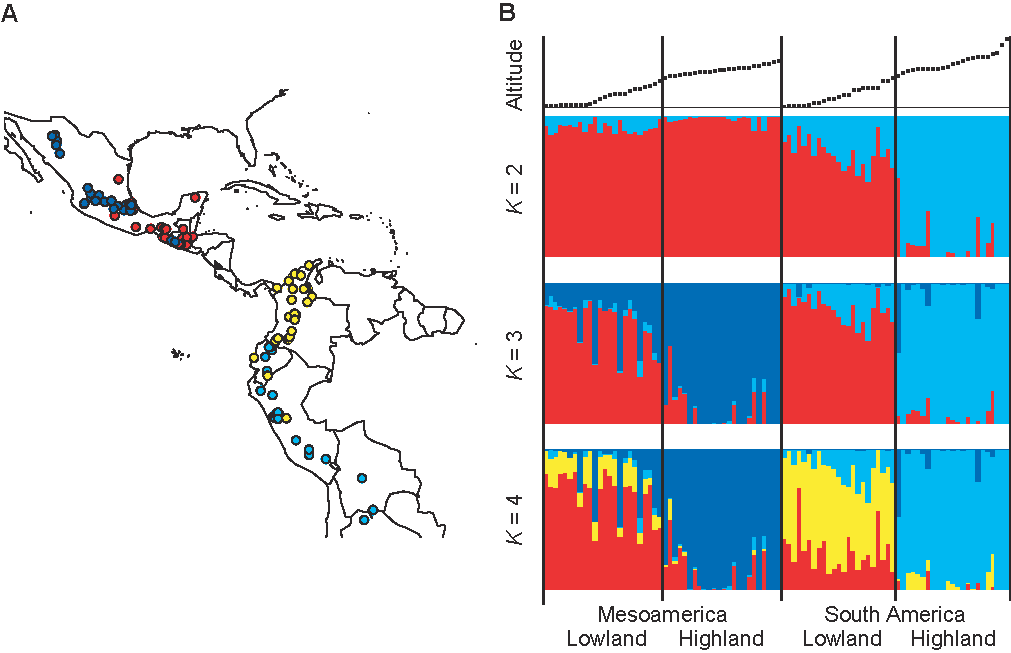
\includegraphics[width=0.8\textwidth]{fig/Fig2}
   \renewcommand{\baselinestretch}{0.9}
   \vspace{-3mm}
   \caption{(A) Sampling locations of landraces.  Red, blue, yellow and light blue dots represent Mexican lowland, Mexican highland, S. American lowland and S. American highland populations, respectively.  (B) Results of {\sf STRUCTURE} analysis of the maizeSNP50 SNPs with $K=2\sim4$.  The top panel shows the altitude, ranging from 0 to 4,000 m on the \emph{y}-axes.  The colors in $K=4$ correspond to those in panel (A).    }
\vspace{-6mm}
    \label{map}
  \end{center}
\end{figure*}
%%%%%%%%%%%%%%%%%%%%%%%%%%%%%%%%%%%%%%%%%% FIGURE

\section*{Materials and Methods}

\subsection*{Materials and DNA extraction}
We included one individual from each of 94 open-pollinated landrace maize accessions from high and low elevation sites in Mexico and S. America (Table \ref{srkid}).   
Accessions were provided by the USDA germplasm repository or kindly donated by Major Goodman (North Carolina State University).  
Sampling locations are shown in Figure~\ref{map}A (see also Table~\ref{srkid}).  
Landraces sampled from altitudes $<1,700$ m were considered lowland, while accessions from $>1,700$ m were considered highland.  
Seeds were germinated on filter paper following fungicide treatment and grown in standard potting mix.  
Leaf tips were harvested from plants at the five leaf stage.  
Following storage at $-80^{\circ}$C overnight, leaf tips were lyophilized for 48 hours.  
Tissue was then homogenized with a Mini-Beadbeater-8 (BioSpec Products, Inc., Bartlesville, OK, USA).  
DNA was extracted using a modified CTAB protocol \cite[]{CTAB}.  
The quality of DNA was ensured through inspection on a 2\% agarose gel and quantification of the ratio of light absorbance at 260 and 280 nm using a NanoDrop spectrophotometer (Thermo Scientific, NanoDrop Products, Wilmington, DE, USA).

\subsection*{SNP data}
We generated two complementary SNP data sets for the sampled maize landraces. 
The first set was generated using the Illumina MaizeSNP50 BeadChip platform, including 56,110 SNPs \cite[]{Ganal_2011_22174790}.  
SNPs were clustered with the default algorithm of the GenomeStudio Genotyping Module v1.0 (Illumina Inc., San Diego, CA, USA).   
Clustering for each SNP was then visually inspected and manually adjusted.  
These data are referred to as "MaizeSNP50" hereafter.  
This array contains SNPs discovered in multiple ascertainment schemes \cite[]{Ganal_2011_22174790}; however, the vast majority of SNPs come from polymorphisms distinguishing the maize inbred lines B73 and Mo17 (14,810 SNPs) or identified from sequencing 25 diverse maize inbred lines \cite[40,594 SNPs;][]{Gore20112009}.  

The second data set was generated for a subset of 87 of the landrace accessions (Table~\ref{srkid}) utilizing high-throughput Illumina sequencing data via genotyping-by-sequencing \cite[GBS;][]{Elshire2011}.
Genotypes were called using TASSEL-GBS \cite[]{Glaubitz_GBS} resulting in 2,848,284 SNPs with an average of 71.3\% missing data per individual.

To assess data quality, we compared genotypes at the 7,197 SNPs (229,937 genotypes, excluding missing data) that overlap between the MaizeSNP50 and GBS data sets. 
While only 0.8\% of 173,670  comparisons involving homozygous MaizeSNP50 genotypes differed in the GBS data, 88.6\% of 56,267 comparisons with MaizeSNP50 heterozygotes differed, nearly always being reported as a homozygote in GBS.
Despite this high heterozygote error rate,  the high correlation in allele frequencies between data sets ($r=0.89$; Figure~\ref{supp:correl_freq}) supports the utility of the GBS data set for estimating allele frequencies.  

We annotated SNPs using the filtered gene set from RefGen version 2 of the maize B73 genome sequence (\citealt{Schnable_2009_19965430}; release 5b.60) from maizesequence.org.  
We excluded genes annotated as transposable elements (84) and pseudogenes (323) from the filtered gene set, resulting in a total of 38,842 genes.

\subsection*{Structure analysis}
We performed a {\sf STRUCTURE} analysis \cite[]{Pritchard_2000_10835412,Falush_2003_12930761} using  synonymous and noncoding SNPs from the MaizeSNP50 data. 
We assumed free recombination between SNPs without missing data and randomly pruned SNPs closer than 10 kb (alternative distances were tried with nearly identical results). 
We excluded SNPs in which the number of heterozygous individuals exceeded homozygotes and where the \emph{P}-value for departure from Hardy-Weinberg Equilibrium (HWE) based on a \emph{G}-test was smaller than 0.05 using all individuals. 
Following these data thinning measures, 17,013 biallelic SNPs remained. 
We conducted three replicate runs of {\sf STRUCTURE} using the correlated allele frequency model with admixture for \emph{K} = 2 through \emph{K} = 6 populations, a burn-in length of 50,000 iterations and a run length of 100,000 iterations. 
Results across replicates were nearly identical.

\subsection*{Demographic inference}
We tested three demographic models in which maize was differentiated into high- and lowland populations subsequent to domestication (Figure~\ref{model}). 
Observed joint frequency distributions (JFDs) were calculated using the GBS data set due to its lower level of ascertainment bias. 
A subset of synonymous and noncoding SNPs were utilized that had $\geq15$ individuals without missing data in both low- and highland populations and did not violate HWE.  
A HWE cut-off of $P<0.005$ was used for each subpopulation due to our under-calling of heterozygotes. 
In total, we included 18,745 silent SNPs for the Mexican populations in Models IA and IB, 14,508 for the S. American populations in Model I and 11,305 for the Mexican lowland population and the S. American populations in Model II.  
We obtained similar results under more or less stringent thresholds for significance ($P < 0.05\sim0.0005$; data not shown), though the number of SNPs was very small at $P<0.005$.  
Demographic parameters were inferred with the software $\delta a \delta i$ \cite[]{Gutenkunst_2009_19851460}, which uses a diffusion method to calculate an expected JFD and evaluates the likelihood of the data using a multinomial assumption.

%%%%%%%%%%%%%%%%%%%%%%%%%%%%%%%%%%%%%%%%%% FIGURE
\begin{figure}[tb]   
  \begin{center}
   \vspace{-0mm}
   %\includegraphics[width=0.23\textwidth]{figs/model}
   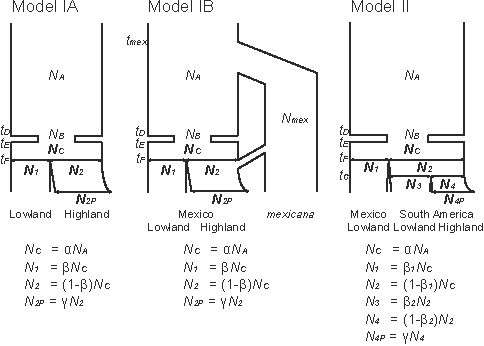
\includegraphics[width=0.5\textwidth]{fig/Fig3}
   \renewcommand{\baselinestretch}{0.9}
   \vspace{-3mm}
   \caption{ Demographic models of maize low- and highland populations.  Parameters in bold were estimated in this study.  See text for details.
   }
\vspace{-6mm}
    \label{model}
  \end{center}
\end{figure}
%%%%%%%%%%%%%%%%%%%%%%%%%%%%%%%%%%%%%%%%%% FIGURE

\subsubsection{Model IA}
This model is applied to the Mexican and S. American populations.
We assume the ancestral diploid population representing \emph{parviglumis} follows a standard Wright-Fisher model with constant size.  
The size of the ancestral population is denoted by $N_A$.
At $t_D$ generations ago, the bottleneck event begins at domestication, and at $t_E$ generations ago, the bottleneck ends.  
The population size and duration of the bottleneck are denoted by $N_B$ and $t_B=t_D-t_E$, respectively.  
The population size recovers to $N_C=\alpha N_A$ in the lowlands.  
Then, the highland population is differentiated from the lowland population at $t_F$ generations ago.  
The size of the low- and highland populations at time $t_F$ is determined by a parameter $\beta$ such that the population is divided by $\beta N_C$ and $(1-\beta)N_C$.  
We assume that the population size in the lowlands is constant but that the highland population experiences exponential expansion after divergence: its current population size is $\gamma$ times larger than that at $t_F$.  \\
%\jri{isn't this really a shrinking population in the lowlands, since $\beta N_C<N_C$ ? wouldn't we want instead for lowlands to stay at $N_C$ and a new population branching off?  how much do we worry about this?}
%\st{actually, our conclusion holds when I assumed the pop size of lowlands stays at $N_C$.  However, the likelihood is a bit better in my original model.}

\subsubsection{Model IB}
We expand Model IA for the Mexican populations by incorporating admixture from the teosinte \emph{mexicana} to the highland Mexican maize population.  
The time of differentiation between \emph{parviglumis} and \emph{mexicana} occurs at $t_{mex}$ generations ago.  
The \emph{mexicana} population size is assumed to be constant at $N_{mex}$.  
At $t_F$ generations ago, the Mexican highland population is derived from admixture between the Mexican lowland population and a portion $P_{mex}$ from the teosinte \emph{mexicana} .  \\

\subsubsection{Model II}
The final model is for the Mexican lowland, S. American lowland and highland populations.  
This model was used for simulating SNPs with ascertainment bias (see below).  
At time $t_F$, the Mexican and S. American lowland populations are differentiated, and the sizes of populations after splitting are determined by $\beta_1$.  
At time $t_G$, S. American lowland and highland populations are differentiated, and the sizes of populations at this time are determined by $\beta_2$.  
As in Model IA, the S. American highland population is assumed to experience population growth with the parameter $\gamma$.\\

Estimates of a number of our model parameters were available from previous work.    
$N_A$ was set to 150,000 using estimates of the composite parameter $4N_A\mu \sim 0.018$ from \emph{parviglumis}  \cite[]{Eyre-Walker_1998_9539756,Tenaillon_2001_11470895,Tenaillon_2004_15014173,Wright_2005_15919994,Ross-Ibarra_2009_19153259} and an estimate of the mutation rate $\mu \sim 3\times 10^{-8}$ \cite[]{Clark_2005_16079248} per site per generation.  
The severity of the domestication bottleneck is represented by $k=N_B/t_B$ \cite[]{Eyre-Walker_1998_9539756,Wright_2005_15919994}, and following \cite{Wright_2005_15919994} we assumed $k=2.45$ and $t_B=1,000$ generations.  
Taking into account archaeological evidence \cite[]{Piperno_2009_19307570}, we assume $t_D=9,000$ and $t_E=8,000$.  
We further assumed $t_F=6,000$ for Mexican populations in Models IA and IB \cite[]{Piperno_2006_69}, $t_F=4,000$ for S. American populations in Model lA \cite[]{Perry_2006_16511492,Grobman_2012_22307642}, and $t_{mex}=60,000$, $N_{mex}=160,000$ \cite[]{Ross-Ibarra_2009_19153259}, and $P_{mex}=0.2$ \cite[]{vanHeerwaarden_2011_21189301} for Model IB. 
For both Models IA and IB, we inferred three parameters ($\alpha$, $\beta$ and $\gamma$), and, for Model II, we fixed $t_F=6,000$ and $t_G=4,000$ \cite[]{Piperno_2006_69,Perry_2006_16511492,Grobman_2012_22307642}  and estimated the remaining four parameters ($\alpha$, $\beta_1$, $\beta_2$ and $\gamma$).

\subsection*{Differentiation between low- and highland populations}
We used our inferred demographic model to generate a null distribution of $F_{ST}$.
As implemented in $\delta a \delta i$ \cite[]{Gutenkunst_2009_19851460}, we calculated an expected JFD given estimated demographic parameters and the sample sizes of highlands and lowlands.
Then, we converted the JFD into the distribution of Fst values.
The \emph{P}-value of a SNP was calculated by $P(F_{ST\_E}\geq F_{ST\_O}|p\pm 0.05) = P(F_{ST\_E}\geq F_{ST\_O} \cap p\pm 0.05)/P(p\pm 0.05)$, 
where $F_{ST\_O}$ and $F_{ST\_E}$ are observed and expected $F_{ST}$ values and $p$ is the mean allele frequency of highlands and lowlands.

Generating the null distribution of differentiation for the MaizeSNP50 data requires accounting for ascertainment bias. 
Evaluation of genetic clustering in our data (not shown) coincides with previous work \cite[]{Hufford_2012_22660546} in suggesting that the two lines most important in the ascertainment panel are most closely related to Mexican lowland maize.  
We thus added two additional individuals to the Mexican lowland population and generated our null distribution using only SNPs for which the two individuals had different alleles.
For model IA in S. America we added two individuals at time $t_F$ to the ancestral population of the S. American low- and highland populations because the Mexican lowland population was not incorporated into this model. 
For each combination of sample sizes in low- and highland populations, we generated a JFD from $10^7$  SNPs using the software {\sf ms} \cite[]{Hudson_2002_11847089}.
Then, we calculated \emph{P}-values from the JDF in the same way.
We calculated $F_{ST}$ values for all SNPs that had $\geq10$ individuals with no missing data in all four populations and showed no departure from HWE at the 0.5\% (GBS) or 5\% (MaizeSNP50) level. 

%\jri{we don't correct for allele frequency (or heterozygosity) in our Fst outlier analysis do we?  if not, this is a problem I think.}
%\st{I did.  No essential change}

%\jri{do we use all GBS data in the Fst outlier test, or just silent SNPs? we should be able to use nonsynonymous too, right?}
%\st{I used all.}

\subsection*{Haplotype sharing test}
We performed a \underline{p}airwise \underline{h}aplotype \underline{s}haring (PHS) test to detect further evidence of selection, following \cite{Toomajian_2006_16623598}.  
To conduct this test, we first imputed and phased the combined SNP data (both GBS and MaizeSNP50) using the {\sf fastPHASE} software version 1.4.0 \cite[]{Scheet_2006_16532393}.  
As a reference for phasing, we used data (excluding heterozygous SNPs) from an Americas-wide sample of 23 partially inbred landraces from the Hapmap v2 data set  \cite[]{Chia_2012_22660545}.  
We ran {\sf fastPHASE}  with default parameter settings.  
PHS was calculated for an allele \emph{A} at position $x$ by

\begin{equation}
  \label{phs-1}
  \begin{array}{l}
  \displaystyle{
PHS_{x_A} = \sum^{p-1}_{i=1}\sum^{p}_{j=i+1}Z_{ijx}  / \Bigl( \begin{array}{c} p \\ 2 \\ \end{array} \Bigr) 
- \sum^{n-1}_{i=1}\sum^{n}_{j=i+1}Z_{ijx}  / \Bigl( \begin{array}{c} n \\ 2 \\ \end{array} \Bigr) 
  }
  \end {array} 
  \textrm{,}
\end{equation}
\noindent where $n$ is sample size of haploids, $p$  is the number of haploids carrying the allele $A$ at position $x$, and

\begin{equation}
  \label{phs-2}
  \begin{array}{l}
  \displaystyle{
Z_{ijx} = \frac{ d_{ijx} - \bar{d_{ij}} }{ \sigma_{ij} }
  }
  \end {array} 
  \textrm{,}
\end{equation}
\noindent where $d_{ijx}$ is the genetic distance over which individuals $i$ and $j$ are identical surrounding position $x$, $\bar{d_{ij}}$ is the genome-wide mean of distances over which individuals are identical, and $\sigma_{ij}$ is the standard deviation of the distribution of distances.  
The \emph{P}-value for each allele was calculated as the proportion of alleles of the same frequency genome-wide that have a larger PHS value. 

Genetic distances were obtained for the MaizeSNP50 data \cite[]{Ganal_2011_22174790} and fit using a tenth degree polynomial curve to all SNPs (data not shown).
 
%JRI STOPPED HERE




%%%% PLR:
\subsection*{Theoretical evaluation of convergent evolution }

We suggest below that many of the high-$F_{ST}$ alleles are locally adaptive,
and the degree of coincidence between highland regions informs us about 
whether these adaptations occurred convergently, 
or if alleles were transmitted between the two by migration.
To see if the abundance and degree of coincidence is consistent with what is known about the population history of maize,
we evaluated the rate at which we expect an allele that provides a selective advantage at higher altitude
to arise by new mutation in a highland region ($\mutrate$),
and the rate at which such an allele already present in the Mexican highlands
would transit the intervening lowlands and fix in the Andean highlands ($\migrate$).
In each case we assume alleles adapted in the highlands are slightly deleterious at lower altitude.  This assumption is consistent with empirical findings in reciprocal transplants of highland and lowland maize in Mexico \cite[]{Mercer2008}.
These numbers depend most strongly on the population density, 
the selection coefficient,
and the rate at which seed is transported long distances and replanted.
We evaluated these rates using new and existing theory, and validated by simulation. Here we describe the mathematical details; readers may skip to the results without loss of continuity.


To calculate the rate at which new mutations appear and fix in a highland population, $\mutrate$,
we multiplied the total population size of the highlands by the mutation rate per generation.
To do this,
we followed \citet{vanHeerwaarden2010} in constructing a detailed demographic model for domesticated maize.
%\plr{this is long-ish?  could perhaps summarize this more/better?}
Fields of $N=10^5$ plants are replanted each year from $N_f=561$ ears,
either from completely new stock (with probability $p_e=0.068$),
from partially new stock (a proportion $r_m=0.2$ with probability $p_m=0.02$),
or entirely from the same field otherwise.
Each plant is seed parent to all kernels of its own ears, but can be pollen parent to kernels in many other ears;
a proportion $m_g=0.0083$ of the pollen-parent kernels are in other fields.
Wild-type plants have an average of $\mu_E=3$ ears per plant, and ears have an average of $N/N_f$ kernels;
each of these numbers are Poisson distributed.
The mean number of pollen-parent kernels, and the mean number of kernels per ear, 
is assumed to be $(1+s_b)$ times larger for individuals heterozygous for the selected allele.
Migration is mediated by seed exchange --
when fields are replanted, the seed is chosen from a random distance away with mean $\sigma_s=50$km,
but plants only pollinate other plants belonging to the same village (distance 0).
Each individual can have offspring in three categories: local seed, local pollen, and migrant seed;
the mean numbers of each of these are determined by the condition that the population is stable
(so wild-type, diploid individuals have on average 2 offspring)
except that heterozygotes have on average $(1+s_b)$ offspring that carry the selected allele.
Each ear has a small chance of being chosen for replanting,
so the number of ears replanted of a given individual is Poisson,
and assuming that pollen is well-mixed, the number of pollen-parent kernels is Poisson as well.
Each of these numbers of offspring has a mean that depends on whether the field is replanted with new stock,
and whether ears are chosen from this field to replant other fields,
so the total number of offspring is actually a mixture of Poissons;
these means, and more details of the computations, are found in Appendix \ref{apx:demographic_model}.

%\plr{got a better term than ``pollen-parent kernels''??}

At these parameter values, we compute that the variance in number of offspring, $\xi^2$, is between 20 (for wild-type) and 30 (for $s_b=0.1$), 
and the dispersal distance (mean distance between parent and offspring)
is $\sigma=1.8$km.

The rate at which new mutations appear and fix in a highland population, which we denote $\mutrate$,
is equal to the total population size of the highlands, multiplied by the mutation rate per generation
and by the chance that a single such mutation successfully fixes
(i.e.\ is not lost to drift).
The latter probability, that a single new mutant allele providing benefit $s_b$ to heterozygotes at high elevation
will fix locally in the high elevation population,
is approximately $2s_b$ divided by the variance in offspring number \citep{jagers1975branching}.
The calculation above is not quite correct, as it neglects migration across the altitudinal gradient,
but exact numerical calculation of the chance of fixation of a mutation as a function of the location where it first appears
indicates that the approximation is quite good (see figure \ref{sfig:prob_estab});
for theoretical treatment see \citet{pollak1966survival} or \citet{barton1987establishment}.

%\plr{could alternatively: (a) describe the math; or (b) cut this down further.}
%I actually like this as is, but think we should expand math as separate appendix. my thinking is math will be of interest to a subset of audience, so perhaps best presented fully but at end. thoughts?
%\plr{added a signpost for non-mathey readers to skip this at the start}

Concretely, the probability that a new mutation destined for fixation
will arise in a patch of high-elevation habitat of area $A$ in a given generation
is a function of the density of maize per unit area $\rho$,
the selective benefit $s_b$ it provides,
the mutation rate $\mu$,
and the variance in offspring number $\xi^2$.
In terms of these parameters, the rate of appearance is
\begin{align} \label{eqn:mutrate}
  \mutrate = \frac{2 \mu \rho A s_b}{\xi^2} .
\end{align}

A corresponding expression for the chance that an allele moves from one highland population to another is harder to intuit,
and is addressed in more depth in \citep{ralphcoop2013patches}.
If an allele is beneficial at high elevation, and fixed in the Mexican highlands,
but deleterious at low elevations,
then it will be present at low frequency in nearby lowland populations,
maintained at migration-selection balance \citep{slatkin1973geneflow}.
This equilibrium frequency decays exponentially with distance,
so that the highland allele is present at distance $R$ from the highlands at frequency $C \exp(- R \sqrt{2s_m} / \sigma)$,
where $s_m$ is the deleterious selection coefficient for the allele in low elevation,
$\sigma$ is the mean dispersal distance,
and $C$ is a constant depending on geography ($C\approx 1/2$ is close).
Multiplying this frequency by a population size gets the predicted number (average density across a large number of generations) of individuals carrying the allele in that population.
Therefore, in a lowland population of size $N$ at distance $R$ from the highlands,
$(N/2)  \exp(- R \sqrt{2s_m} / \sigma)$ is equal to the probability that there are any highland alleles present,
multiplied by the expected number of these, given that there are some present.
Since the latter is at least 1,
%don't follow. "latter" is expected number? why is that at least one? didn't you say above it could be 0<x<1 because it's an average density?
the chance there are any present in a given generation is no more than $(N/2) \exp(- R \sqrt{2s_m} / \sigma)$,
and so this puts an upper bound on $\migrate$.
Therefore, we would need to wait $\Tmig = (2/N)\exp(R \sqrt{2s_m} / \sigma)$ generations 
for a rare such excursion to occur.
In other words, we can bound the rate of migration by
\begin{align}
  \migrate \le (N/2)  \exp(- R \sqrt{2s_m} / \sigma) ,
\end{align}
with $N$ being the total size of the unadapted highland population,
and $R$ the distance from the adapted to the yet-unadapted highland populations.
This also omits the probability that such an allele fixes ($\approx 2s_b/\xi^2$), 
but since such alleles arrive by migration, this omission is unlikely a large effect and is conservative.

To obtain specific predictions,
we then computed $\mutrate$ and $\migrate$ at various parameter values.
We also checked these with simulations and more detailed computations,
described in the Appendix.



